% ═══════════════════════════════════════════════════════════════════════
\section{Images, tableaux et figures}
% ═══════════════════════════════════════════════════════════════════════

\begin{frame}[fragile]{Insérer une image}
  \begin{columns}[c]
    \begin{column}{0.58\textwidth}
\begin{CodeTeX}[title={Avec graphicx}]
\begin{figure}[h]
  \centering
  \includegraphics[width=0.5\textwidth]{triangle.png}
  \caption{Un triangle rectangle.}
\end{figure}
\end{CodeTeX}
    \end{column}
    \begin{column}{0.39\textwidth}
      \small
      \begin{enumerate}
        \item Téléverser l'image dans le projet Overleaf (icône
          Téléverser, au-dessus de la liste des fichiers).
        \item Écrire son nom exact, avec l'extension.
        \item Régler la taille par \texttt{width=}, en fraction de la
          largeur du texte.
      \end{enumerate}
    \end{column}
  \end{columns}
  \vspace{4pt}
  \small \texttt{figure} numérote l'image et la place au mieux dans la
  page ; \texttt{[h]} demande « ici, si possible ».
\end{frame}

\begin{frame}[fragile]{Un tableau de valeurs}
\begin{CodeRendu}[title={L'environnement tabular}]
\begin{tabular}{c|ccccc}
  $x$    & $-2$ & $-1$ & $0$ & $1$ & $2$ \\
  \hline
  $f(x)$ & $4$  & $1$  & $0$ & $1$ & $4$
\end{tabular}
\end{CodeRendu}
  \small
  \begin{itemize}
    \item \texttt{\{c|ccccc\}} : une colonne par lettre (\texttt{l}, \texttt{c},
      \texttt{r} : à gauche, centrée, à droite) ; \texttt{|} trace un
      trait vertical.
    \item \texttt{\&} sépare les colonnes, \texttt{\textbackslash\textbackslash} termine
      une ligne, \cmd{hline} trace un trait horizontal.
    \item Pour un grand tableau, l'IA fait gagner beaucoup de temps.
  \end{itemize}
\end{frame}

\begin{frame}[fragile]{Dessiner avec TikZ}
\begin{CodeRendu}[title={Un triangle rectangle}]
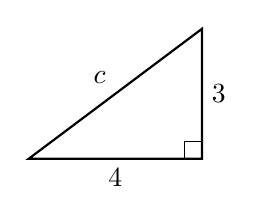
\begin{tikzpicture}[scale=0.55]
  \draw[thick] (0,0) -- (4,0)
        -- (4,3) -- cycle;
  \draw (3.6,0) |- (4,0.4);
  \node[below] at (2,0) {$4$};
  \node[right] at (4,1.5) {$3$};
  \node[above left] at (2,1.5) {$c$};
\end{tikzpicture}
\end{CodeRendu}
  \small
  \begin{itemize}
    \item On décrit la figure par des coordonnées : \texttt{(4,3)} est le
      point d'abscisse $4$ et d'ordonnée $3$.
    \item L'IA produit très bien du TikZ ; votre travail : ajuster une
      coordonnée, une étiquette, une échelle --- à la main.
  \end{itemize}
\end{frame}
